\section{Results}
\subsection*{Bayesian Model}

Diagnostic plots for Bayesian model fit to the real apixaban data is shown in \cref{fig:fig3}.  Posterior population prediction intervals (that is, the result of integrating out the random effect of each patient) of the observed concentration are realistic and to the eye appear similar to the observed data (top left of \cref{fig:fig3}).  Residual plots (observed minus posterior mean) indicate homogeneity of variance on the log scale, which is consistent both with expert knowledge on the measurement process and the likelihood we choose (bottom left of \cref{fig:fig3}). Predicted concentrations tend to agree with observed concentrations (top right of \cref{fig:fig3}), and posterior predictive draws have similar empirical cumulative distribution functions as the observed data (bottom right of \cref{fig:fig3} ). In \cref{fig:fig4}, we show concentration functions obtained from draws from our prior distribution as well as two patients with best and worst fit as measured by mean absolute percent error (best: 3.29\%, worst: 26.4\%). Because our HMC diagnostics do not indicate problematic behaviour in the Markov chains, and because the model diagnostics indicate adequate fit, we believe the obtained model’s posterior predictive distribution is adequate for simulation of pseudopatients.


\begin{figure}
	\centering
	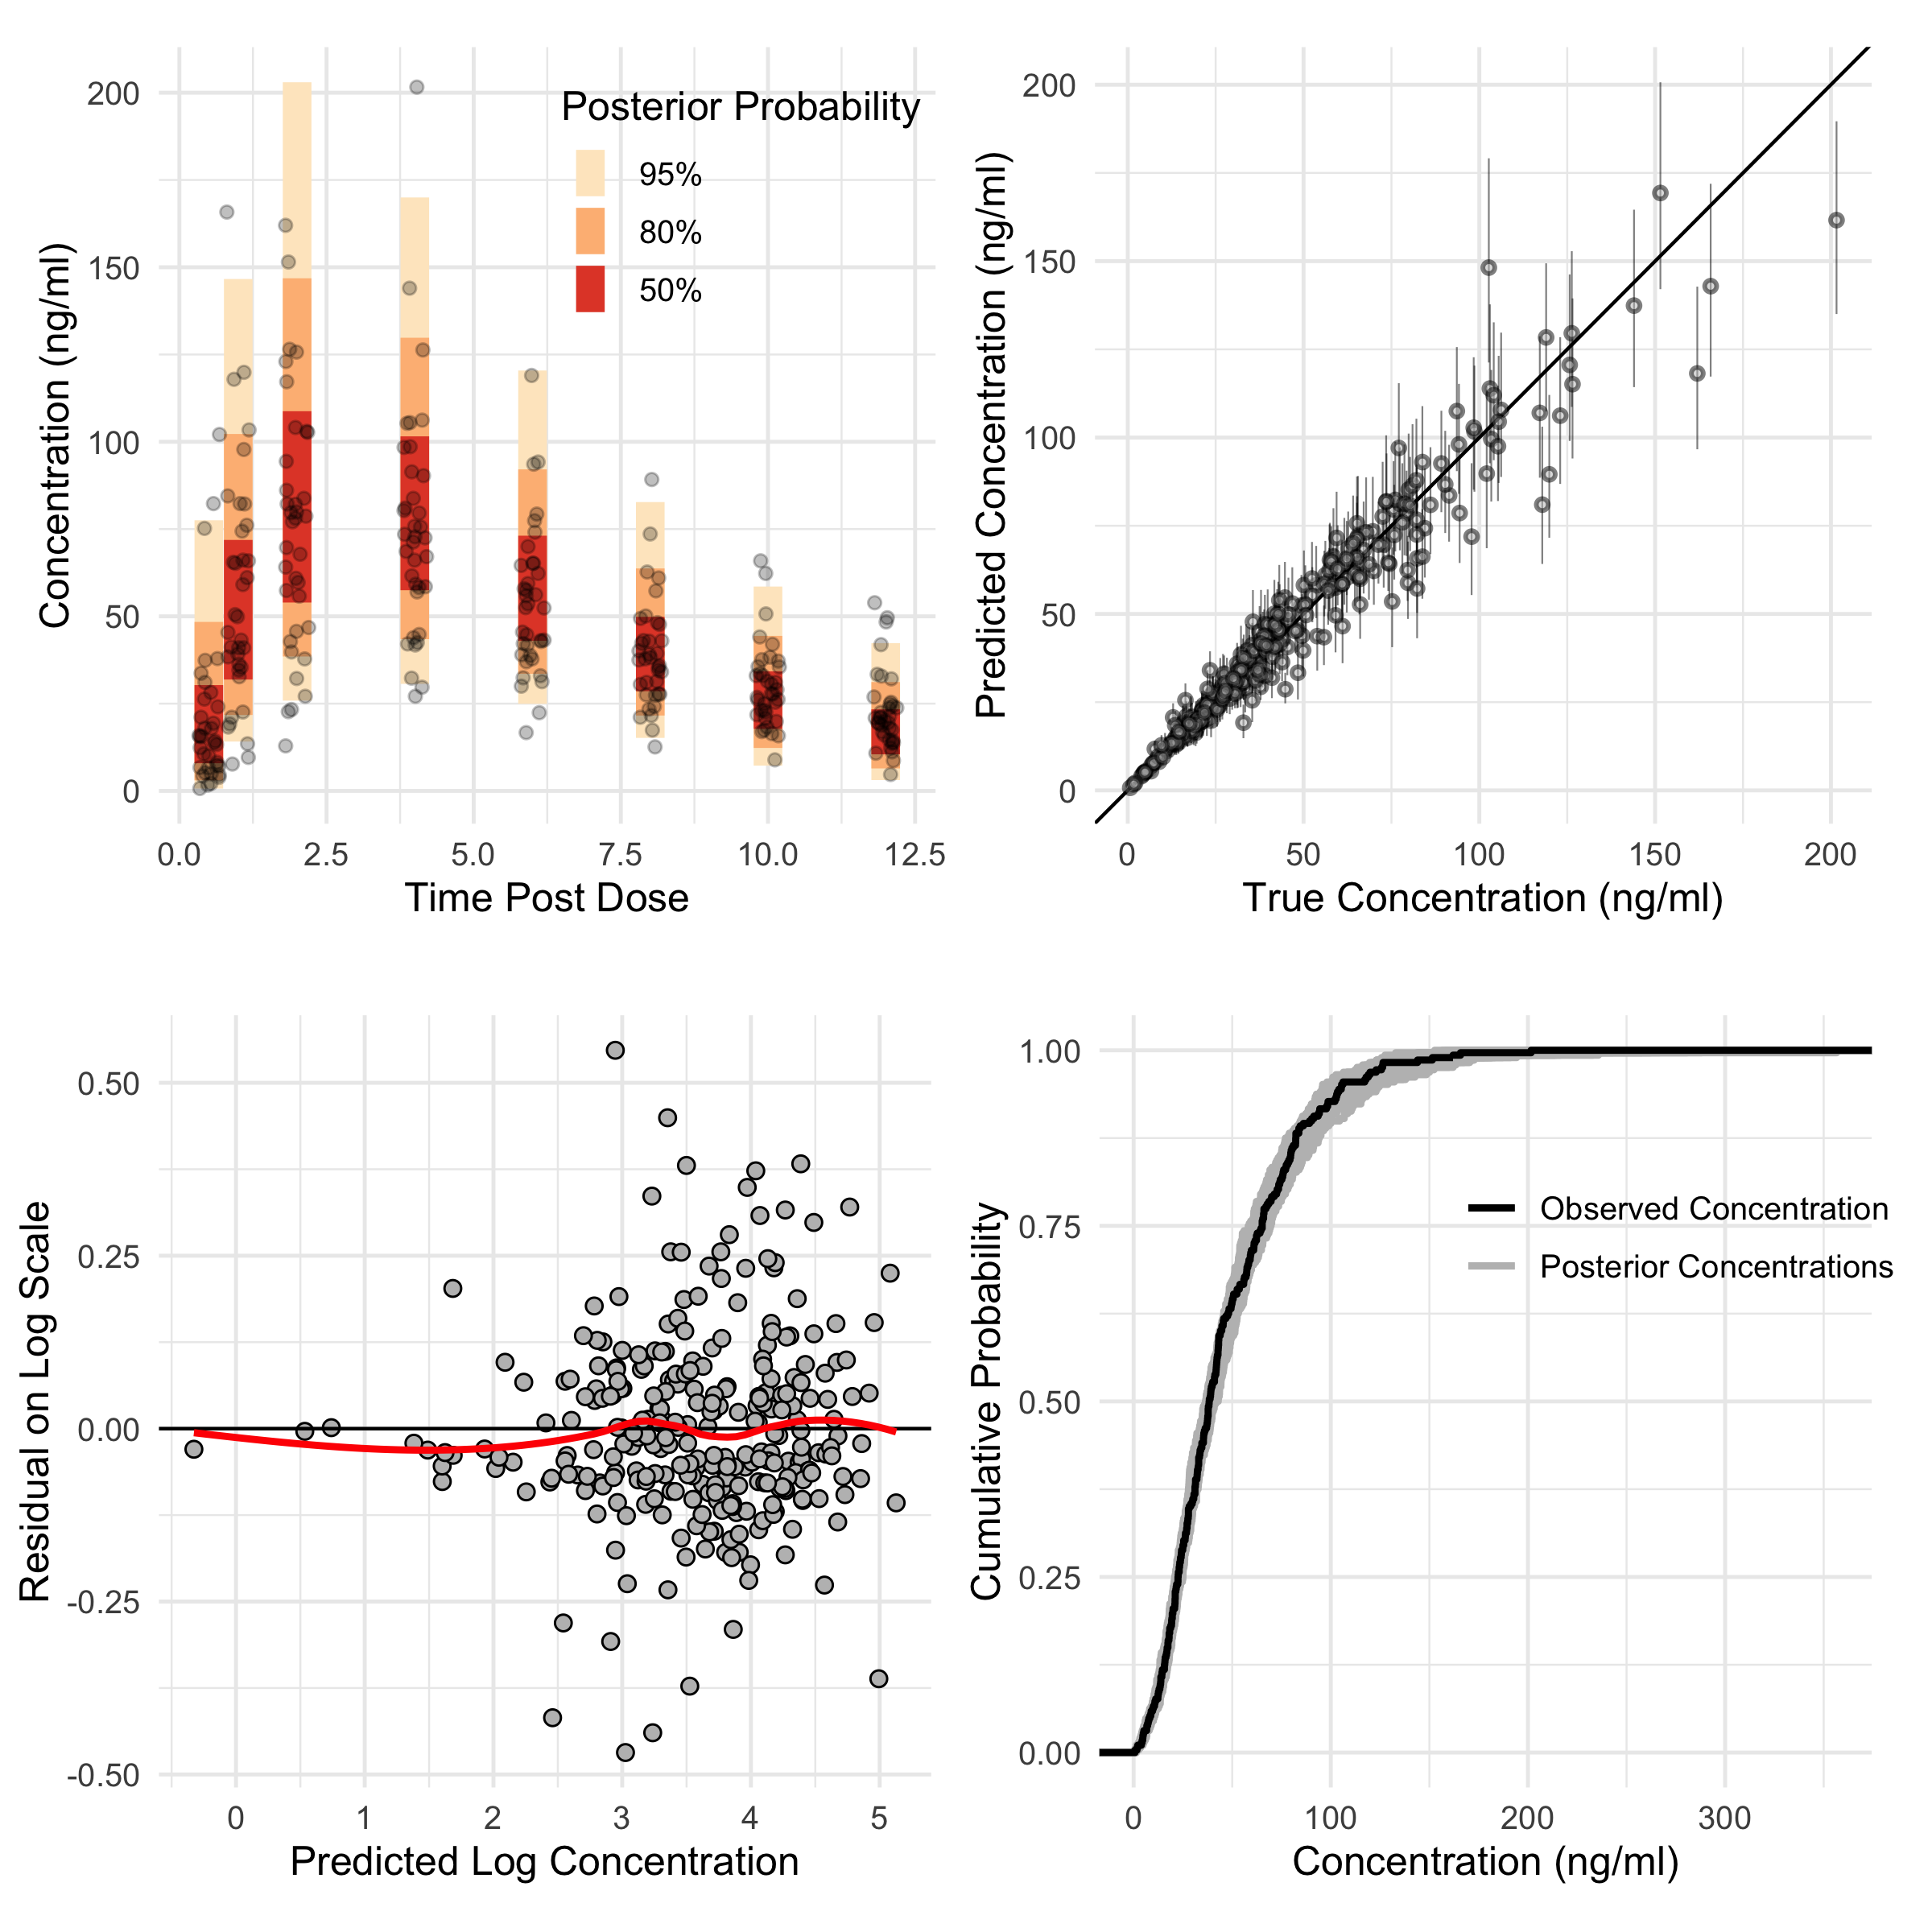
\includegraphics[width=0.9\linewidth]{figs/diagnostics}
	\caption{Diagnostic plots for our Bayesian model.  Top left shows the posterior predictive distribution plus observed data.  Data points gave been perturbed to prevent overlapping. Top right shows the predicted values along with accompanying 95\% equal-tailed posterior credible interval. Bottom left shows the residuals (on the log scale) between the observed concentrations and the posterior mean concentration, bottom right shows the cumulative density function for the observed data (black) as well as draws from the posterior predictive distribution (gray).}
	\label{fig:fig3}
\end{figure}


\begin{figure}
	\centering
	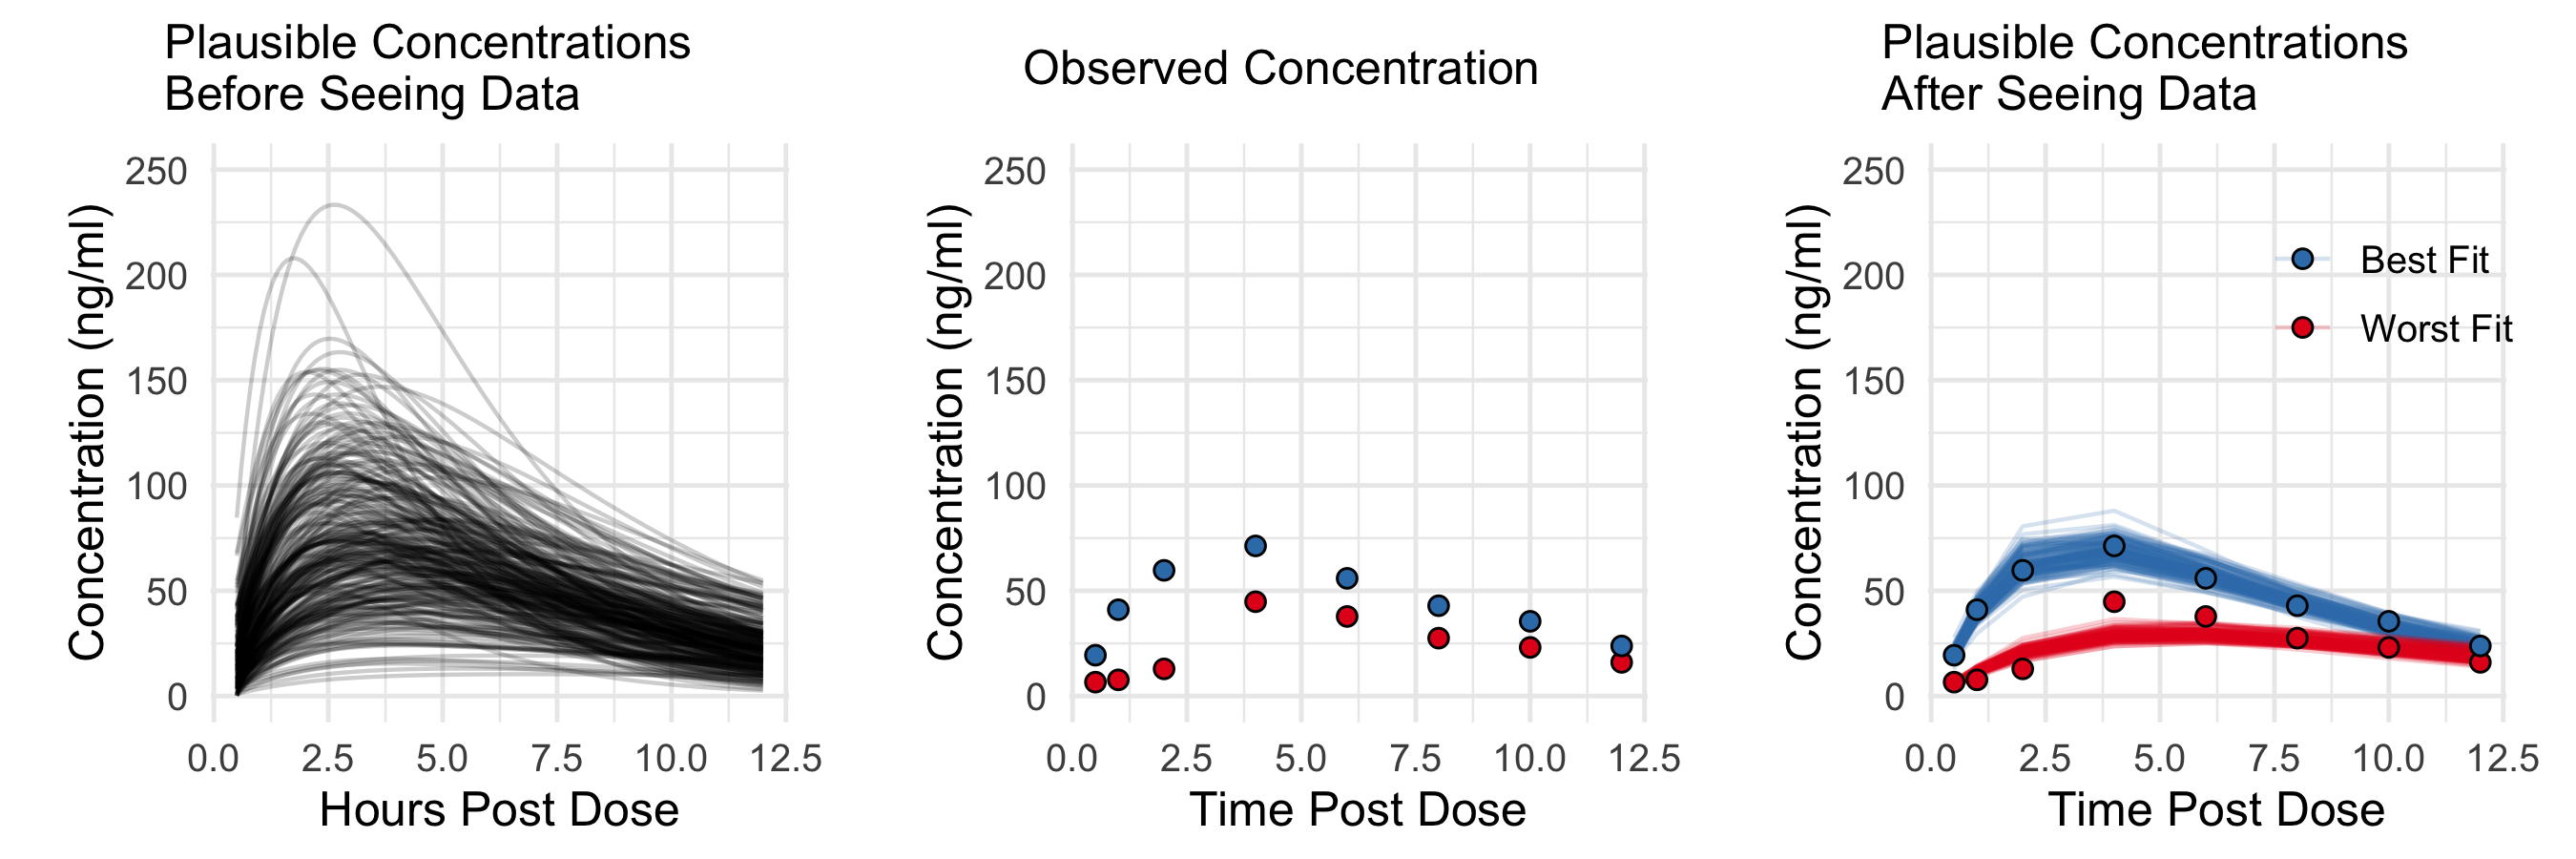
\includegraphics[width=\linewidth]{figs/fig3}
	\caption{The leftmost panel shows 250 draws from the prior defined in the previous section.  The center panel shows data from two patients who acieved the best (blue) and worst (red) model fit as measured through mean absolute percent error.  The rightmost panel shows 250 draws from the posterior for these patients.  Not shown here are the other 34 patients in our data, for which the model is also capable of performing predictions for. }
	\label{fig:fig4}
\end{figure}

\begin{figure}
	\centering
	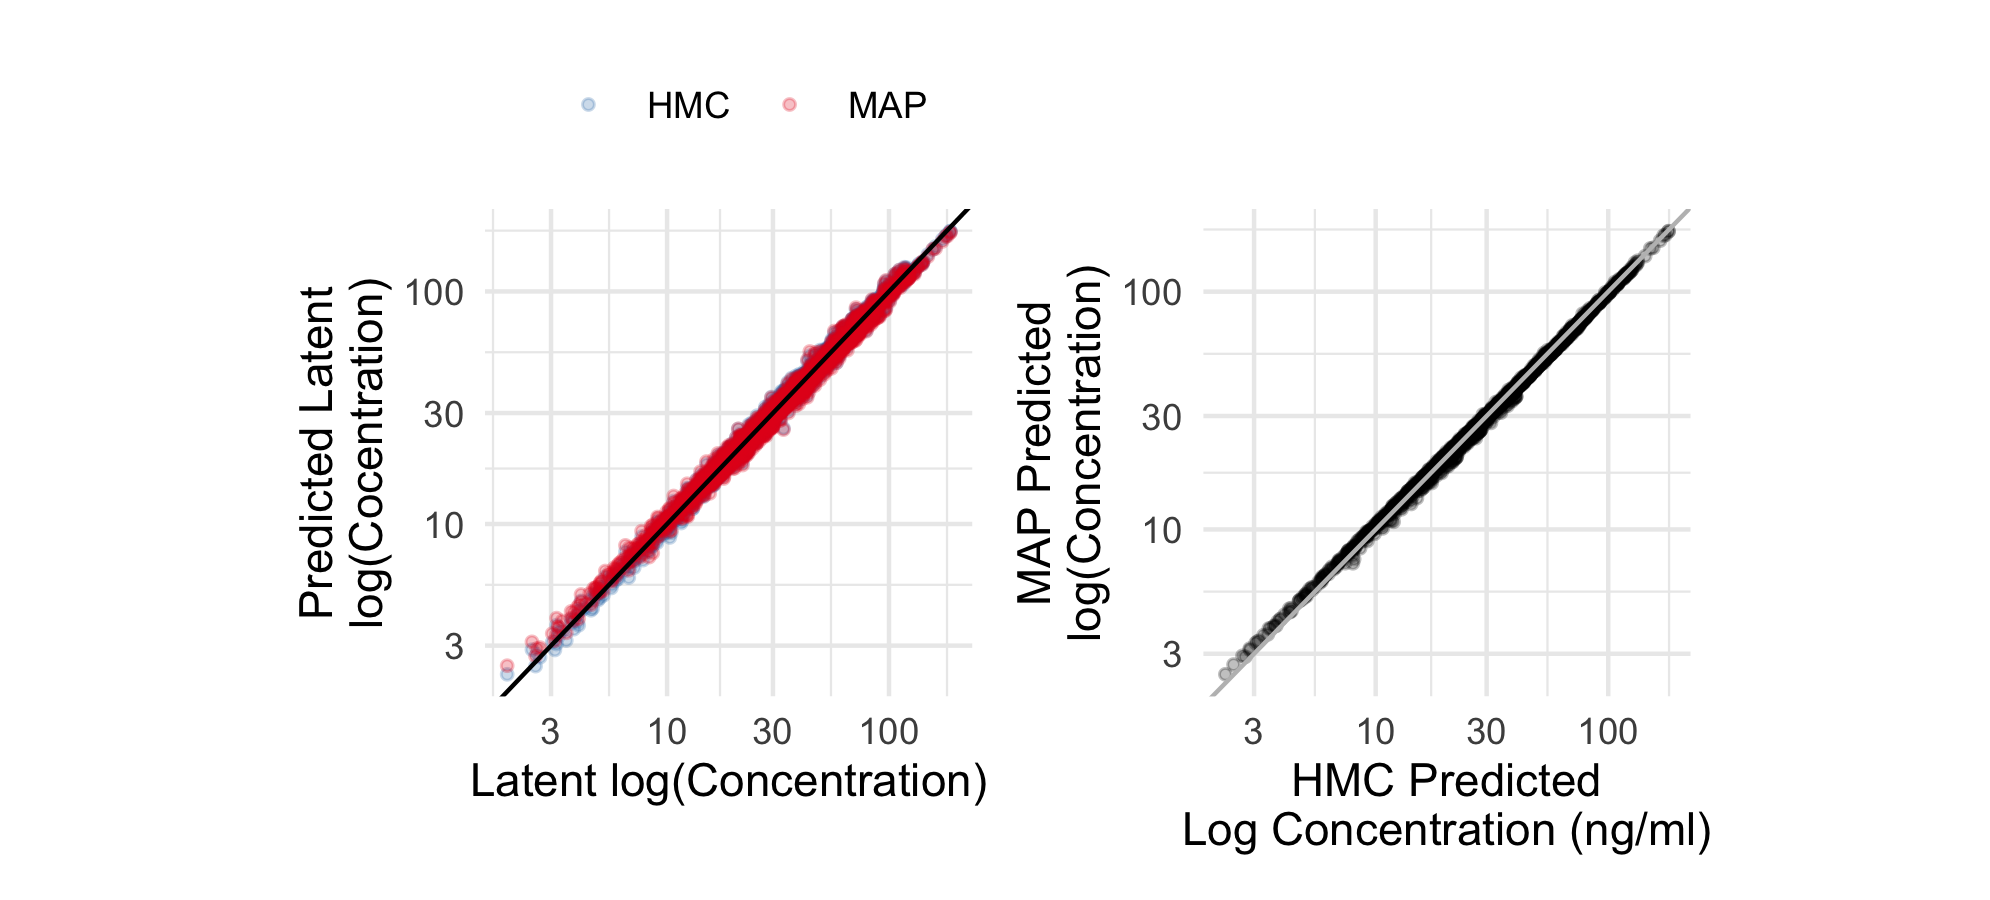
\includegraphics[width=1\linewidth]{figs/compare}
	\caption{Comparisons of fits obtained through HMC and MAP for simulated patients.  On the left, the two methods are compared to the true concentration values, and on the right the two methods are compared to one another.  The predictions are negligibly different to the eye and are also negligibly different as compared by Mean Squared Error (MSE), Mean Absolute Error (MAE), and Mean Absolute Percentage Error (MAPE).}
	\label{fig:fig5}
\end{figure}



\subsection*{Fit on Simulated Patients Using HMC and MAP}

Initial comparisons of predicted values indicate that both HMC and MAP yield similar predictions to one another, and similar predictions to actual values of unseen data.  Examining predictions alone, it would seem that HMC and MAP are equivalent, or at the very least similar enough so as to not have strong preference for one over the other. When using posterior means, HMC results in lower prediction error on unseen data as measured with Mean Squared Error (MSE), Mean Absolute Error (MAE), and Mean Absolute Percentage Error (MAPE), but these are not stark differences. Estimates of posterior uncertainty between MAP and HMC can however vary a great deal. Shown in \cref{fig:fig6} are 19 of the 100 simulated patients which have a MAP equal tailed posterior interval at least 50\% larger as compared to their HMC equal tail posterior interval at the widest point. We note that while not shown explicitly, unobserved concentrations lie entirely within the HMC and MAP posterior intervals.



\begin{table}
	\centering
\begin{tabular}{|c|c|c|}
	\hline 
	& HMC & MAP \\ 
	\hline 
	MSE (SD) & 6.67 (15.93) & 8.57 (19.93) \\ 
	\hline 
	MAE (SD) & 1.71 (1.94) & 1.97 (2.17) \\ 
	\hline 
	MAPE (SD) & 0.04 (0.03) & 0.05 (0.03)\\ 
	\hline 
\end{tabular} 
\caption{Comparison of HMC and MAP on three loss functions common in pharmacokinetics:  Mean Squared Error (MSE), Mean Absolute Error (MAE), and Mean Absolute Percentage Error (MAPE).  The loss was computed on samples not seen by our model.  Included in parentheses are the standard deviations of the loss values.}
\end{table}

%\begin{figure}
%	\centering
%	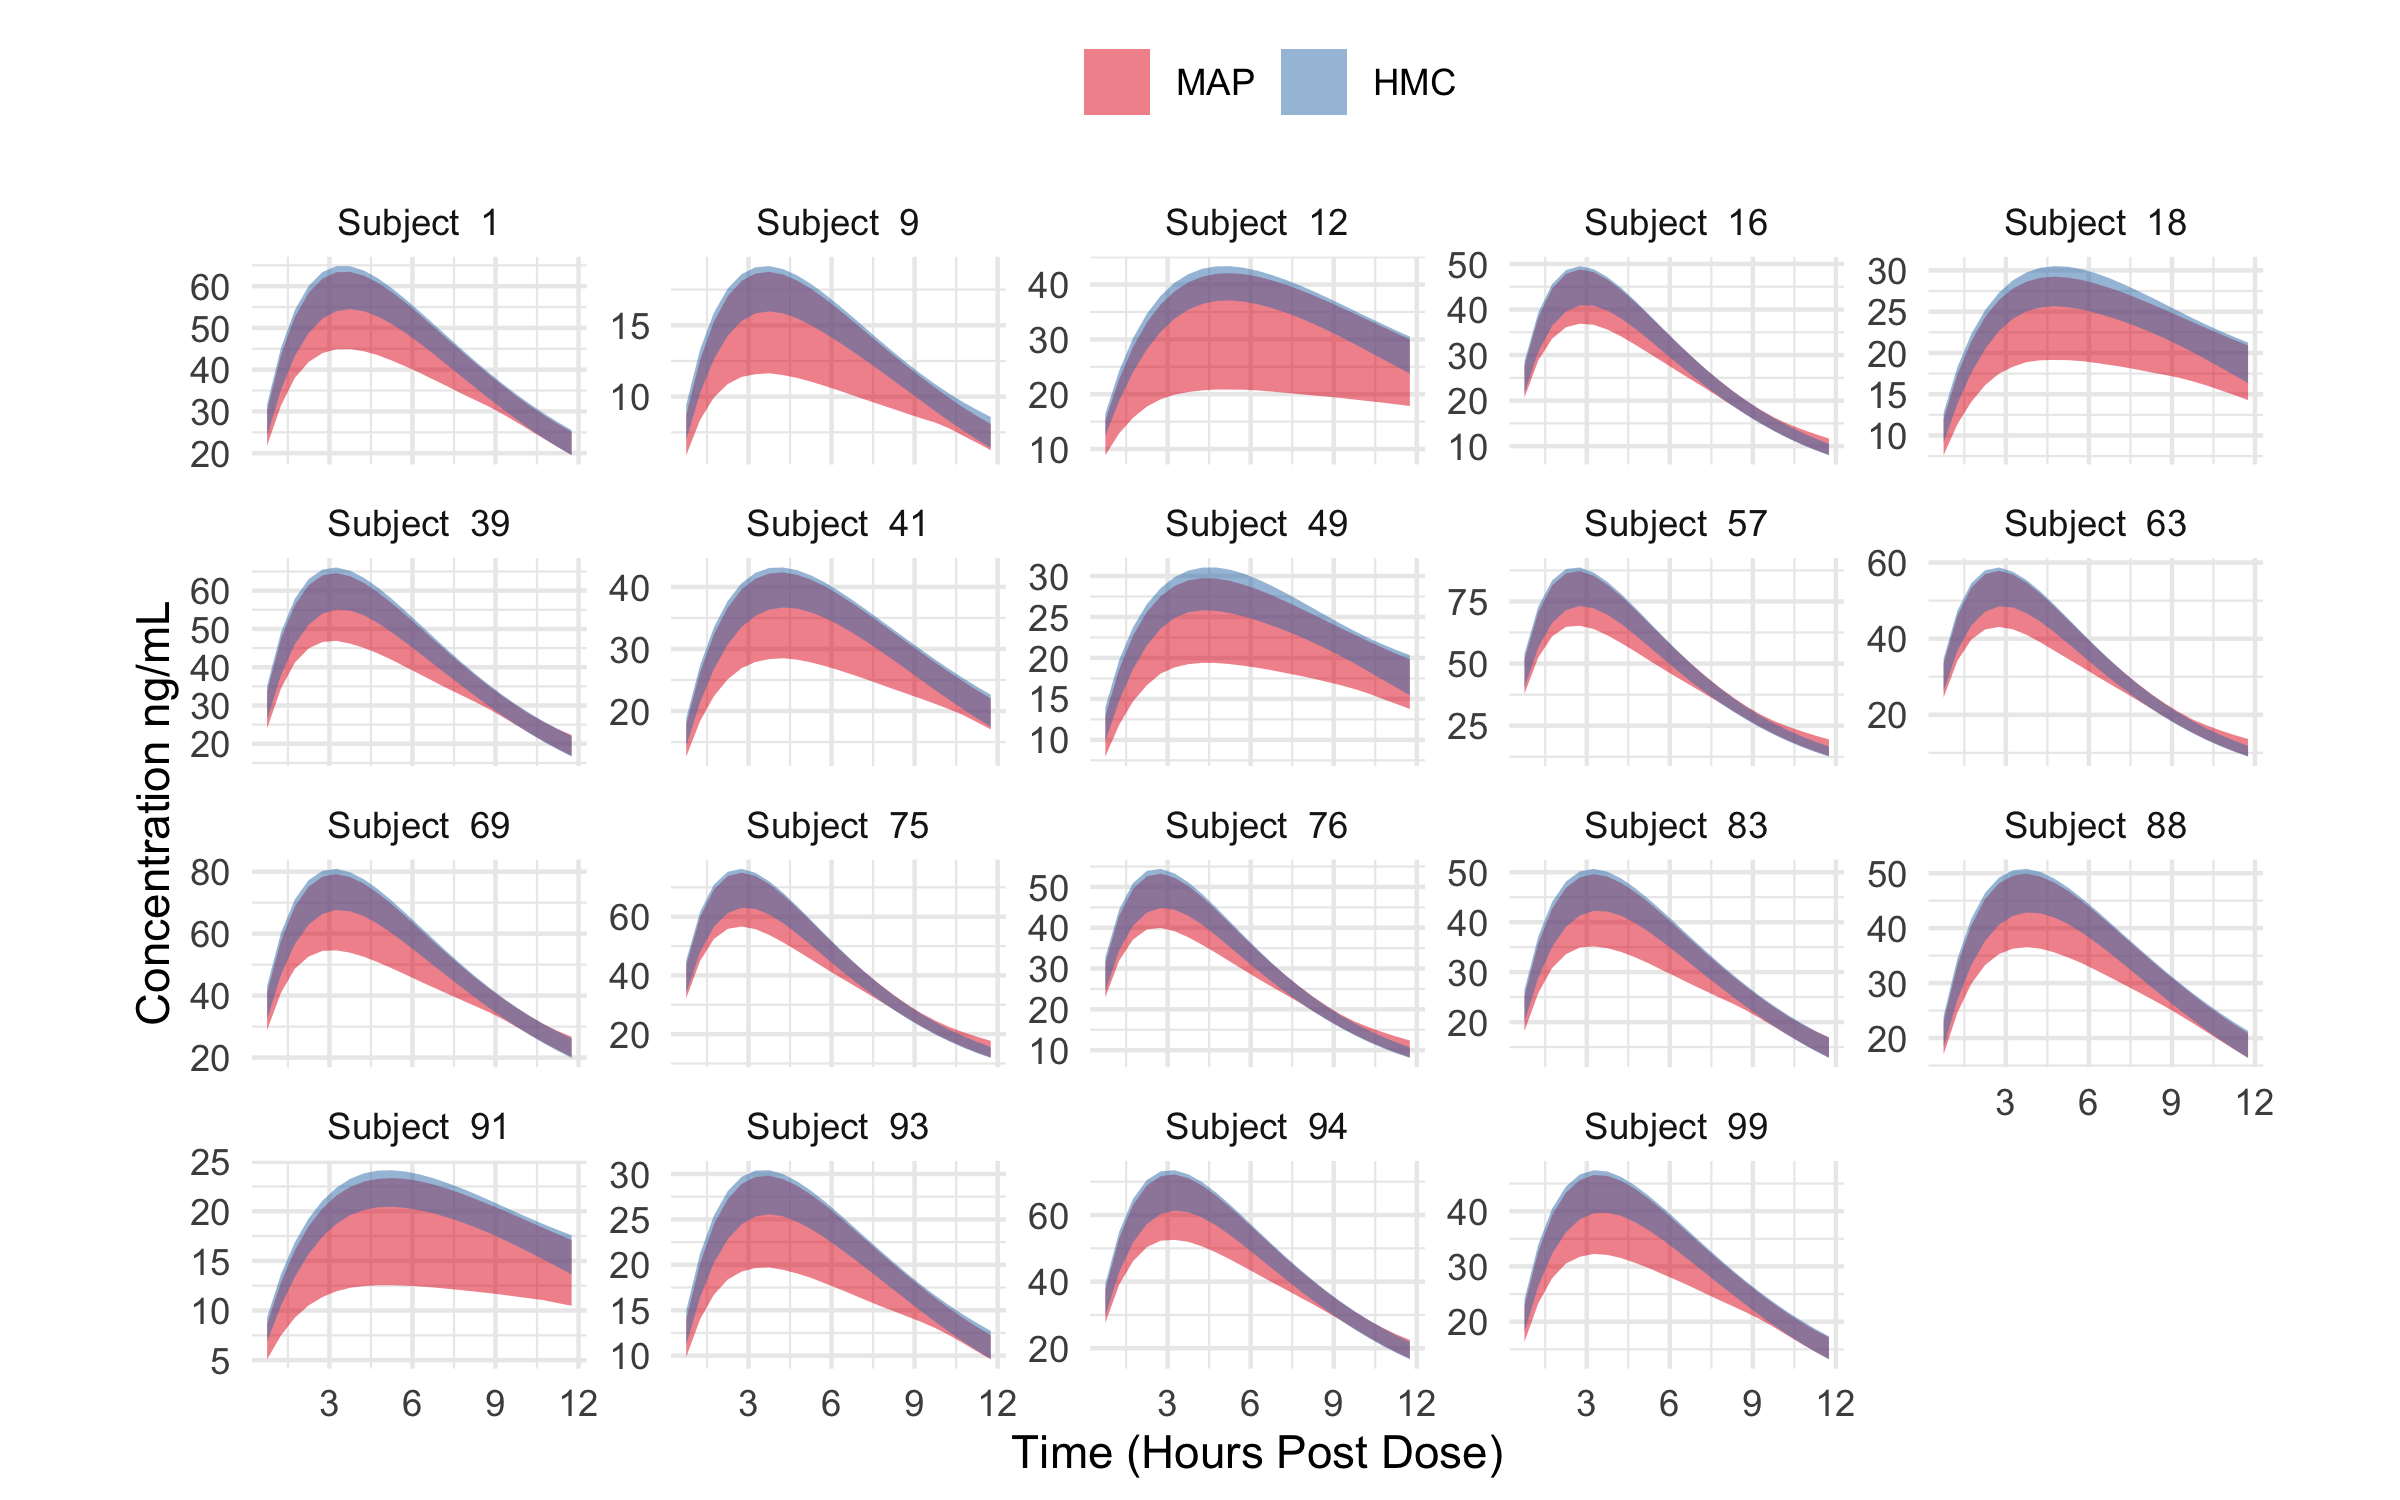
\includegraphics[width=1\linewidth]{figs/intervals}
%	\caption{Comparisons of equal tail posterior intervals from MAP and HMC. Note that the concentration scales differ from subplot to subplot.  Selected patients are those which have a MAP posterior interval at least 50\% as wide or wider than their HMC interval.  In many simulated subjects.}
%	\label{fig:fig6}
%\end{figure}
\clearpage
\begin{sidewaysfigure}[h!]
\centering
	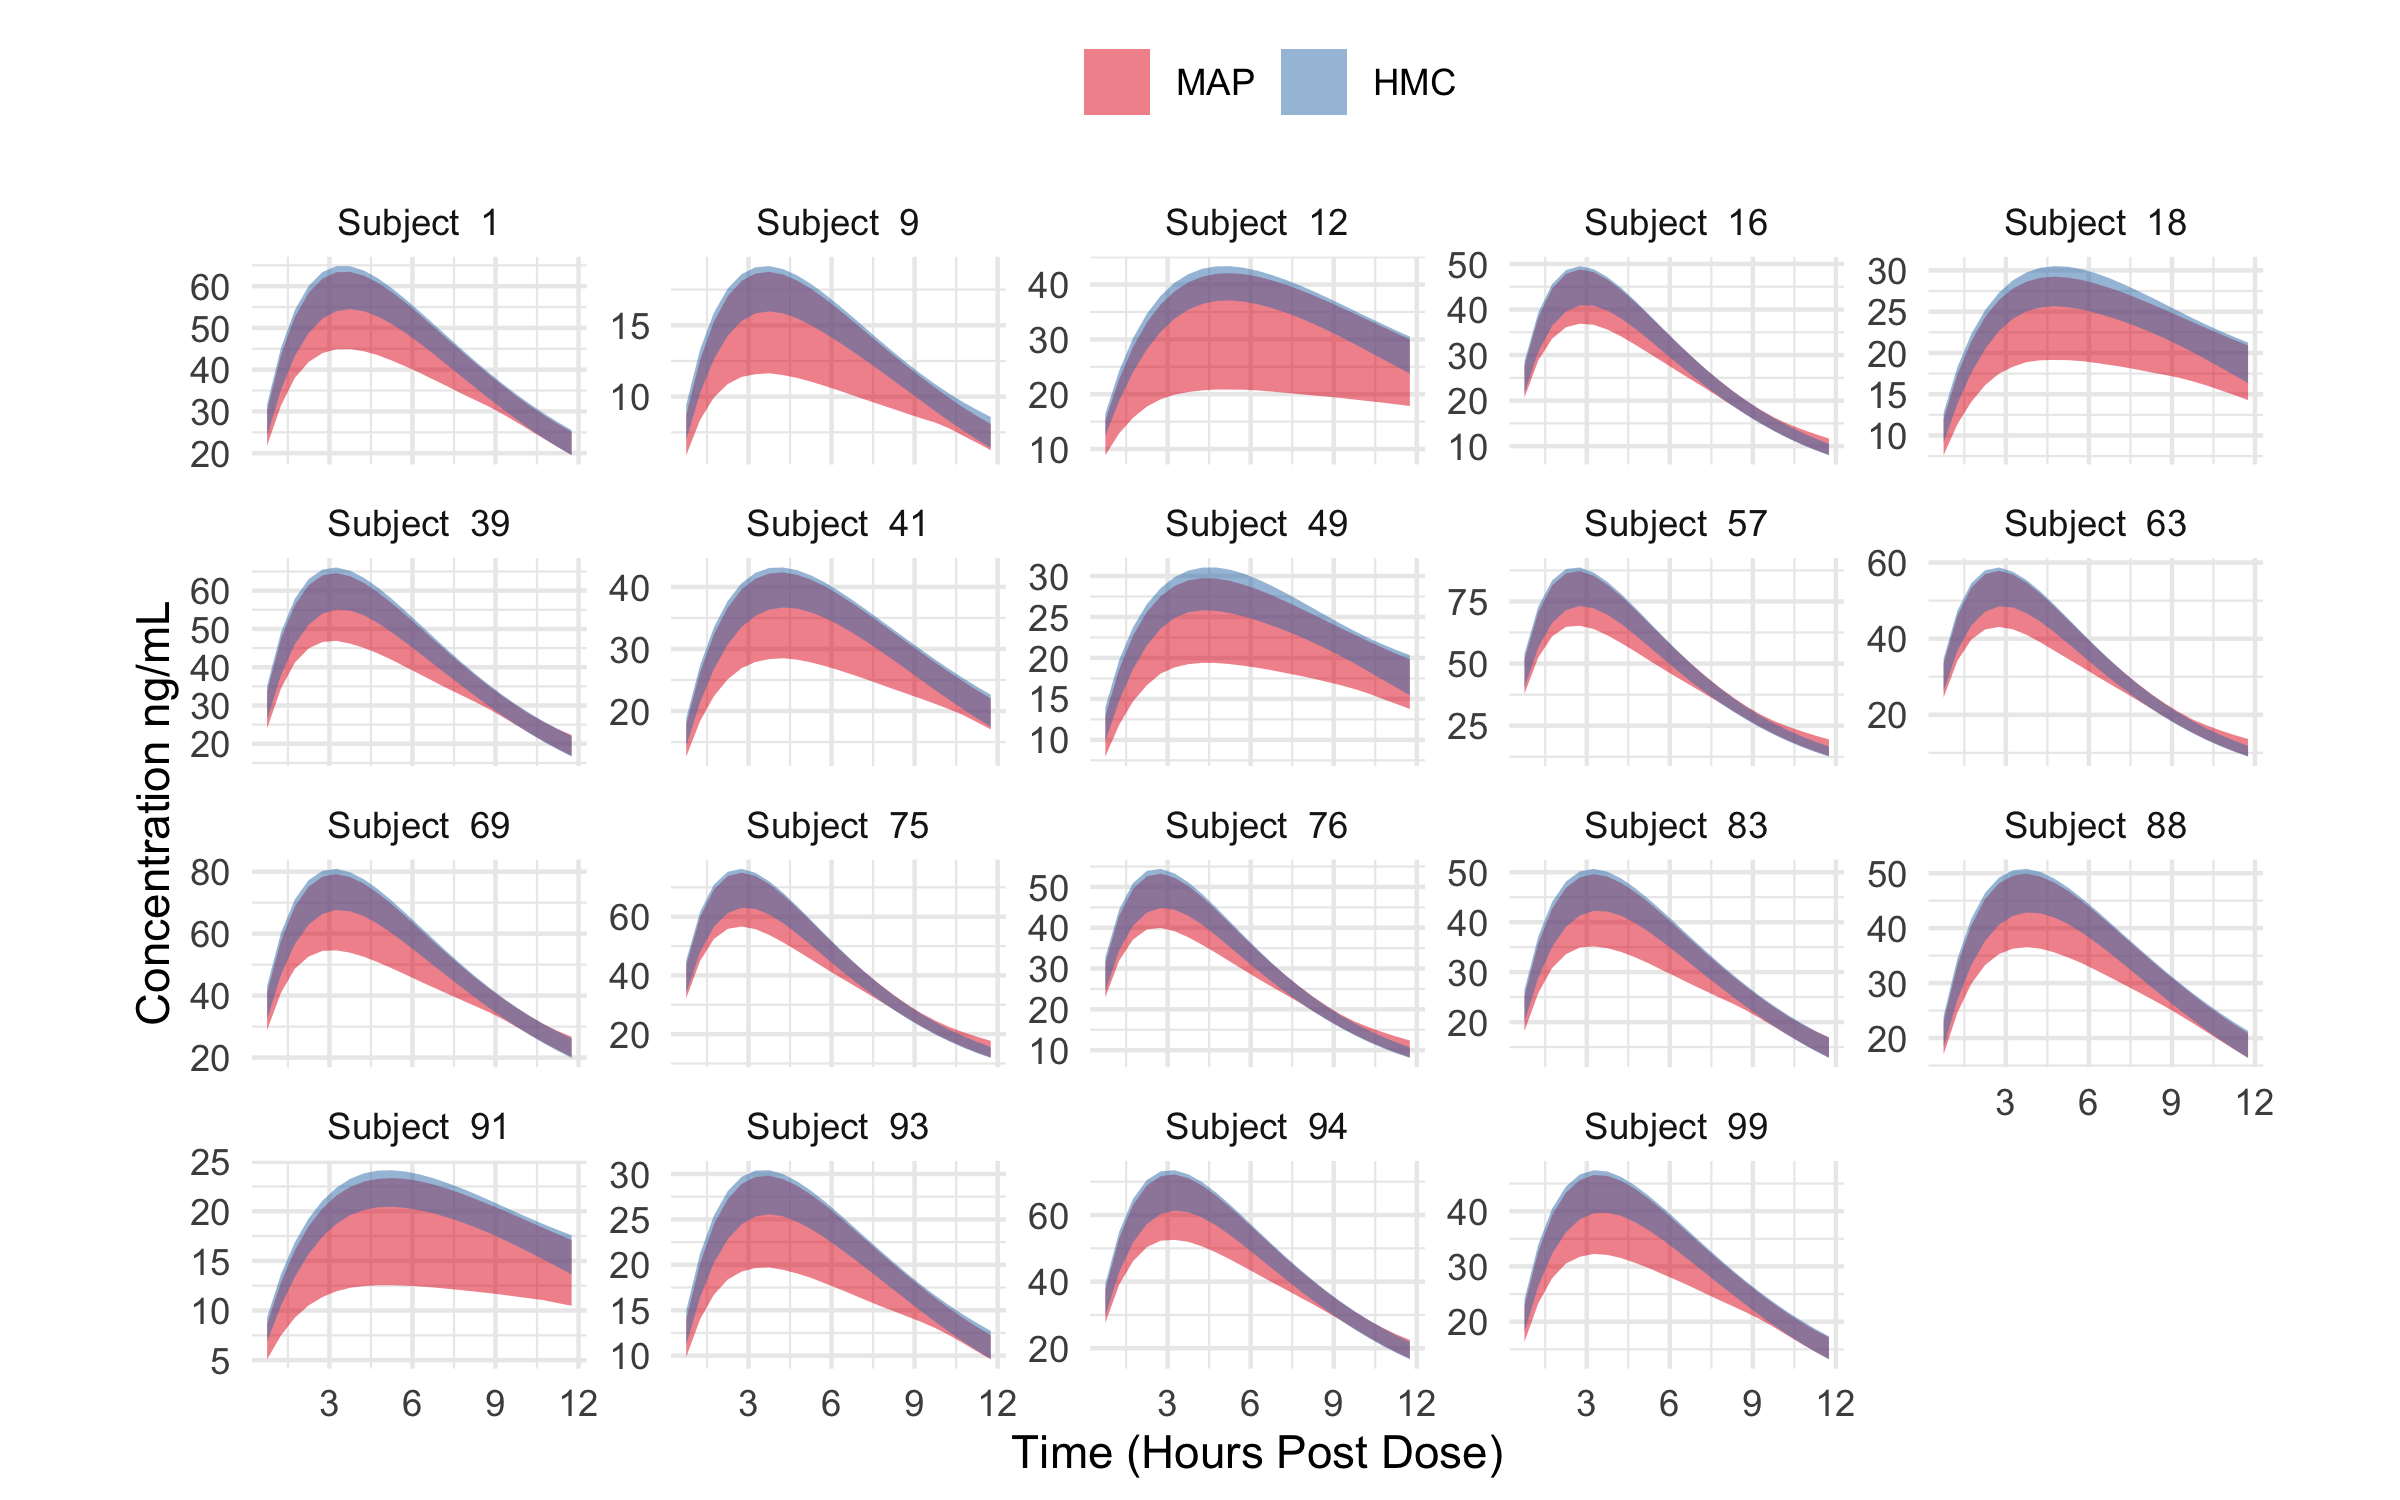
\includegraphics[width=1\linewidth]{figs/intervals}
	\caption{Comparisons of equal tail posterior intervals from MAP and HMC. Note that the concentration scales differ from subplot to subplot.  Selected patients are those which have a MAP posterior interval at least 50\% as wide or wider than their HMC interval.  In many simulated subjects.}
	\label{fig:fig6}
\end{sidewaysfigure}
\clearpage

\subsection*{Difference in Estimated Dose To Achieve Target Risk}


By inverting the risk curve, we can obtain dose size as a function of risk.  Shown in \cref{fig:fig7} are the differences between doses computed from HMC and MAP posteriors to achieve the indicated level of risk.  The left panel shows the difference in doses in order to achieve a concentration of at least 20 ng/ml 12 hours post dose. For a majority of patients, MAP and HMC agree to within 1 mg though some pseudopatients see a much larger dose recommendation by HMC than by MAP.  The right panel shows the difference in doses in order to achieve a max concentration of 80 ng/ml.  MAP tends to always recommend larger doses than HMC for this scenario, with the difference between recommended doses becoming larger as the desired risk becomes smaller.

\begin{figure}[h!]
	\centering
	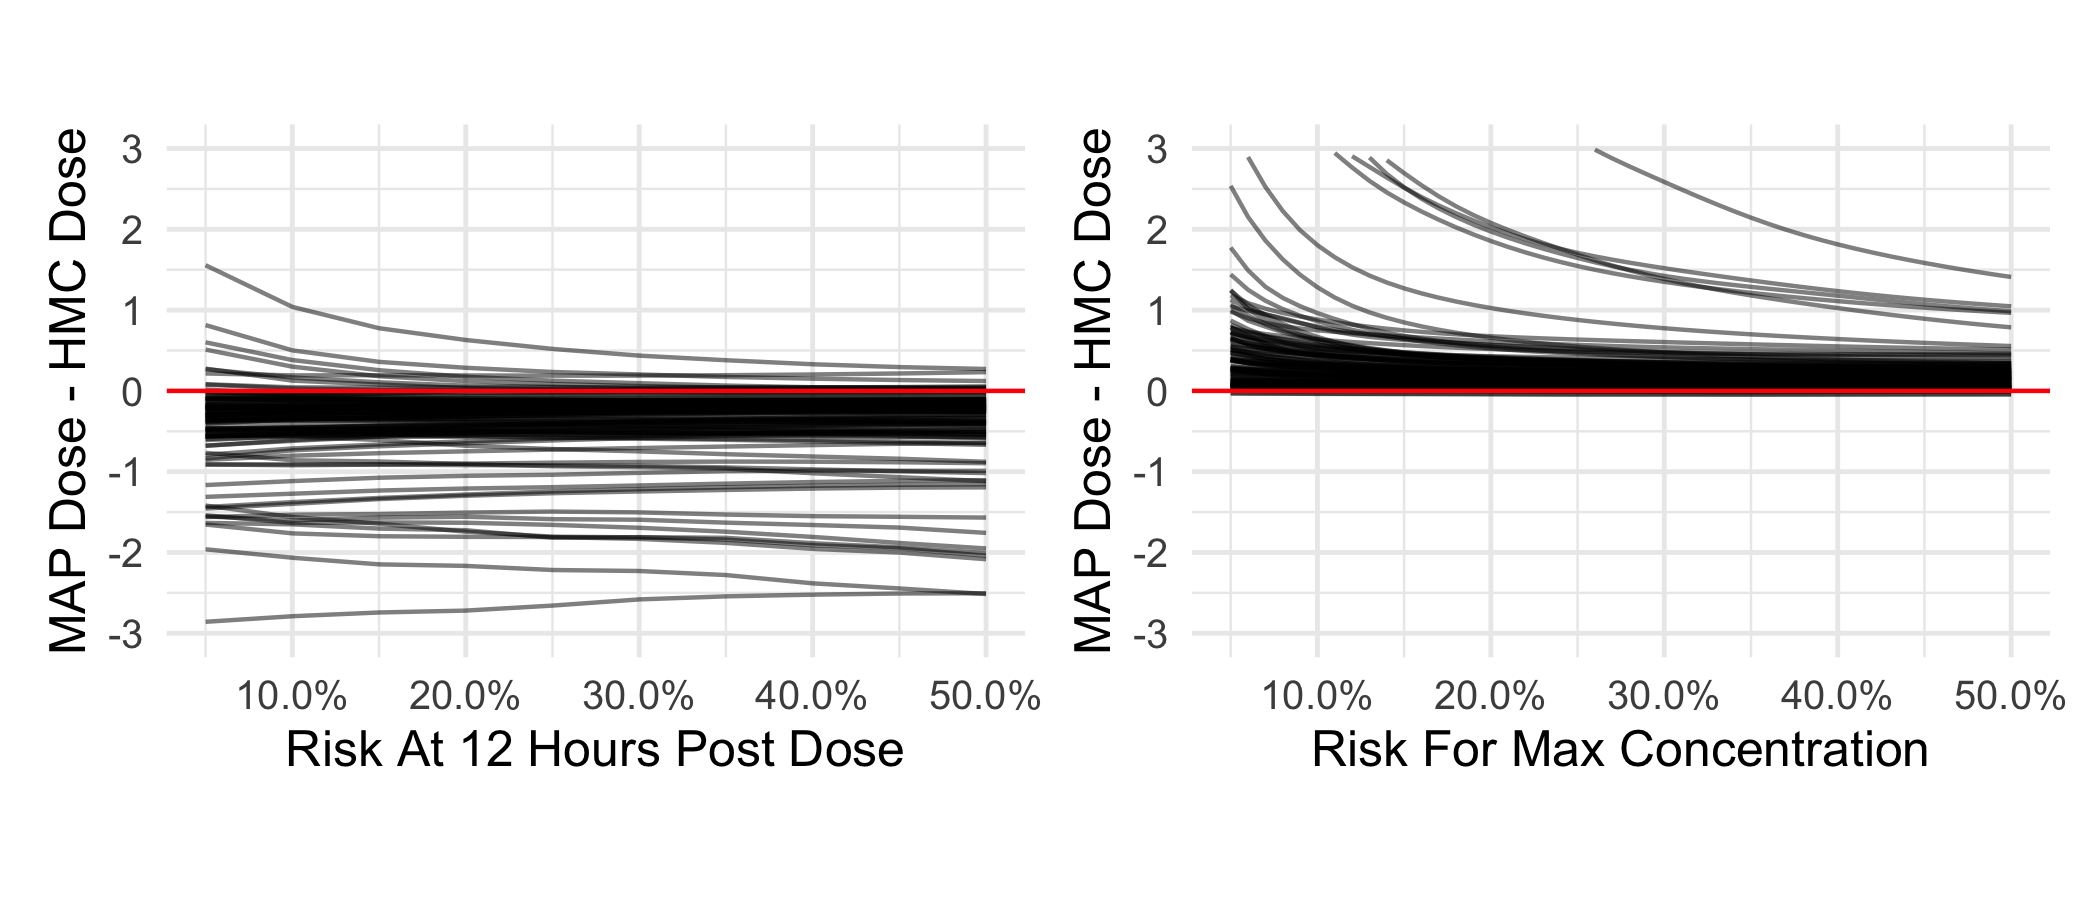
\includegraphics[width=\linewidth]{figs/experiments}
	\caption{Left: Differences between the estimated doses from MAP and HMC to achieve the indicated risk of having a concentration of apixiban smaller than 20 ng/ml at 12 hours post dose. Each line corresponds to one of the 100 pseudopatients. MAP tends to recommend larger doses than HMC to achieve a desired risk of having the patient's concentration at 12 hours post dose be below 20 ng/ml. This tendency to recommend larger doses is consistent across desired risk levels.  Right: Differences between estimated doses from MAP and HMC to achieve the indicated risk of having a max concentration smaller than 80 ng/ml.  Some pseudopatients see dose recommendation differences as large as 10 mg and are thus cut off by the y axis limits. Red lines indicate perfect agreement between the two methods.}
	\label{fig:fig7}
\end{figure}


\subsection*{Calibration for Dosing Decisions}

Since all pseudopatients were simulated, the true concentration function as a function of the dose size (\cref{eq:eq_1}) was known.  To further compare HMC and MAP for decision making, we took estimated dose size to achieve a desired risk and computed what the concentration curve under the recommended dose size.  We could then compute the number of pseudopatients which actually exceeded the threshold, thus allowing us to examine the calibration of HMC and MAP.  The calibration curves for HMC and MAP for both experiments are shown in \cref{fig:fig8}

In the first experiment (left of \cref{fig:fig8}), HMC is better calibrated than MAP.  This means that when a dose is selected, in order to a achieve a risk of being below 20 ng/ml at 12 hours post dose of $r$, approximately $r \times 100$ pseudopatients have a true concentration function which is smaller than 20 ng/ml at 12 hours post dose. In contrast, MAP is poorly calibrated, and sees more pseudopatients failing to exceed the 20 ng/ml threshold than was desired.  Calibration in our second experiment again shows than HMC is better calibrated than MAP, but calibration seems to become worse as the desired risk becomes larger.  When we use dose sizes recommended by MAP to achieve a 50\% probability of exceeding the 80 ng/ml threshold, only 26\% of pseudopatients actually have a max concentration which exceeds the threshold.


\begin{figure}[h!]
	\centering
	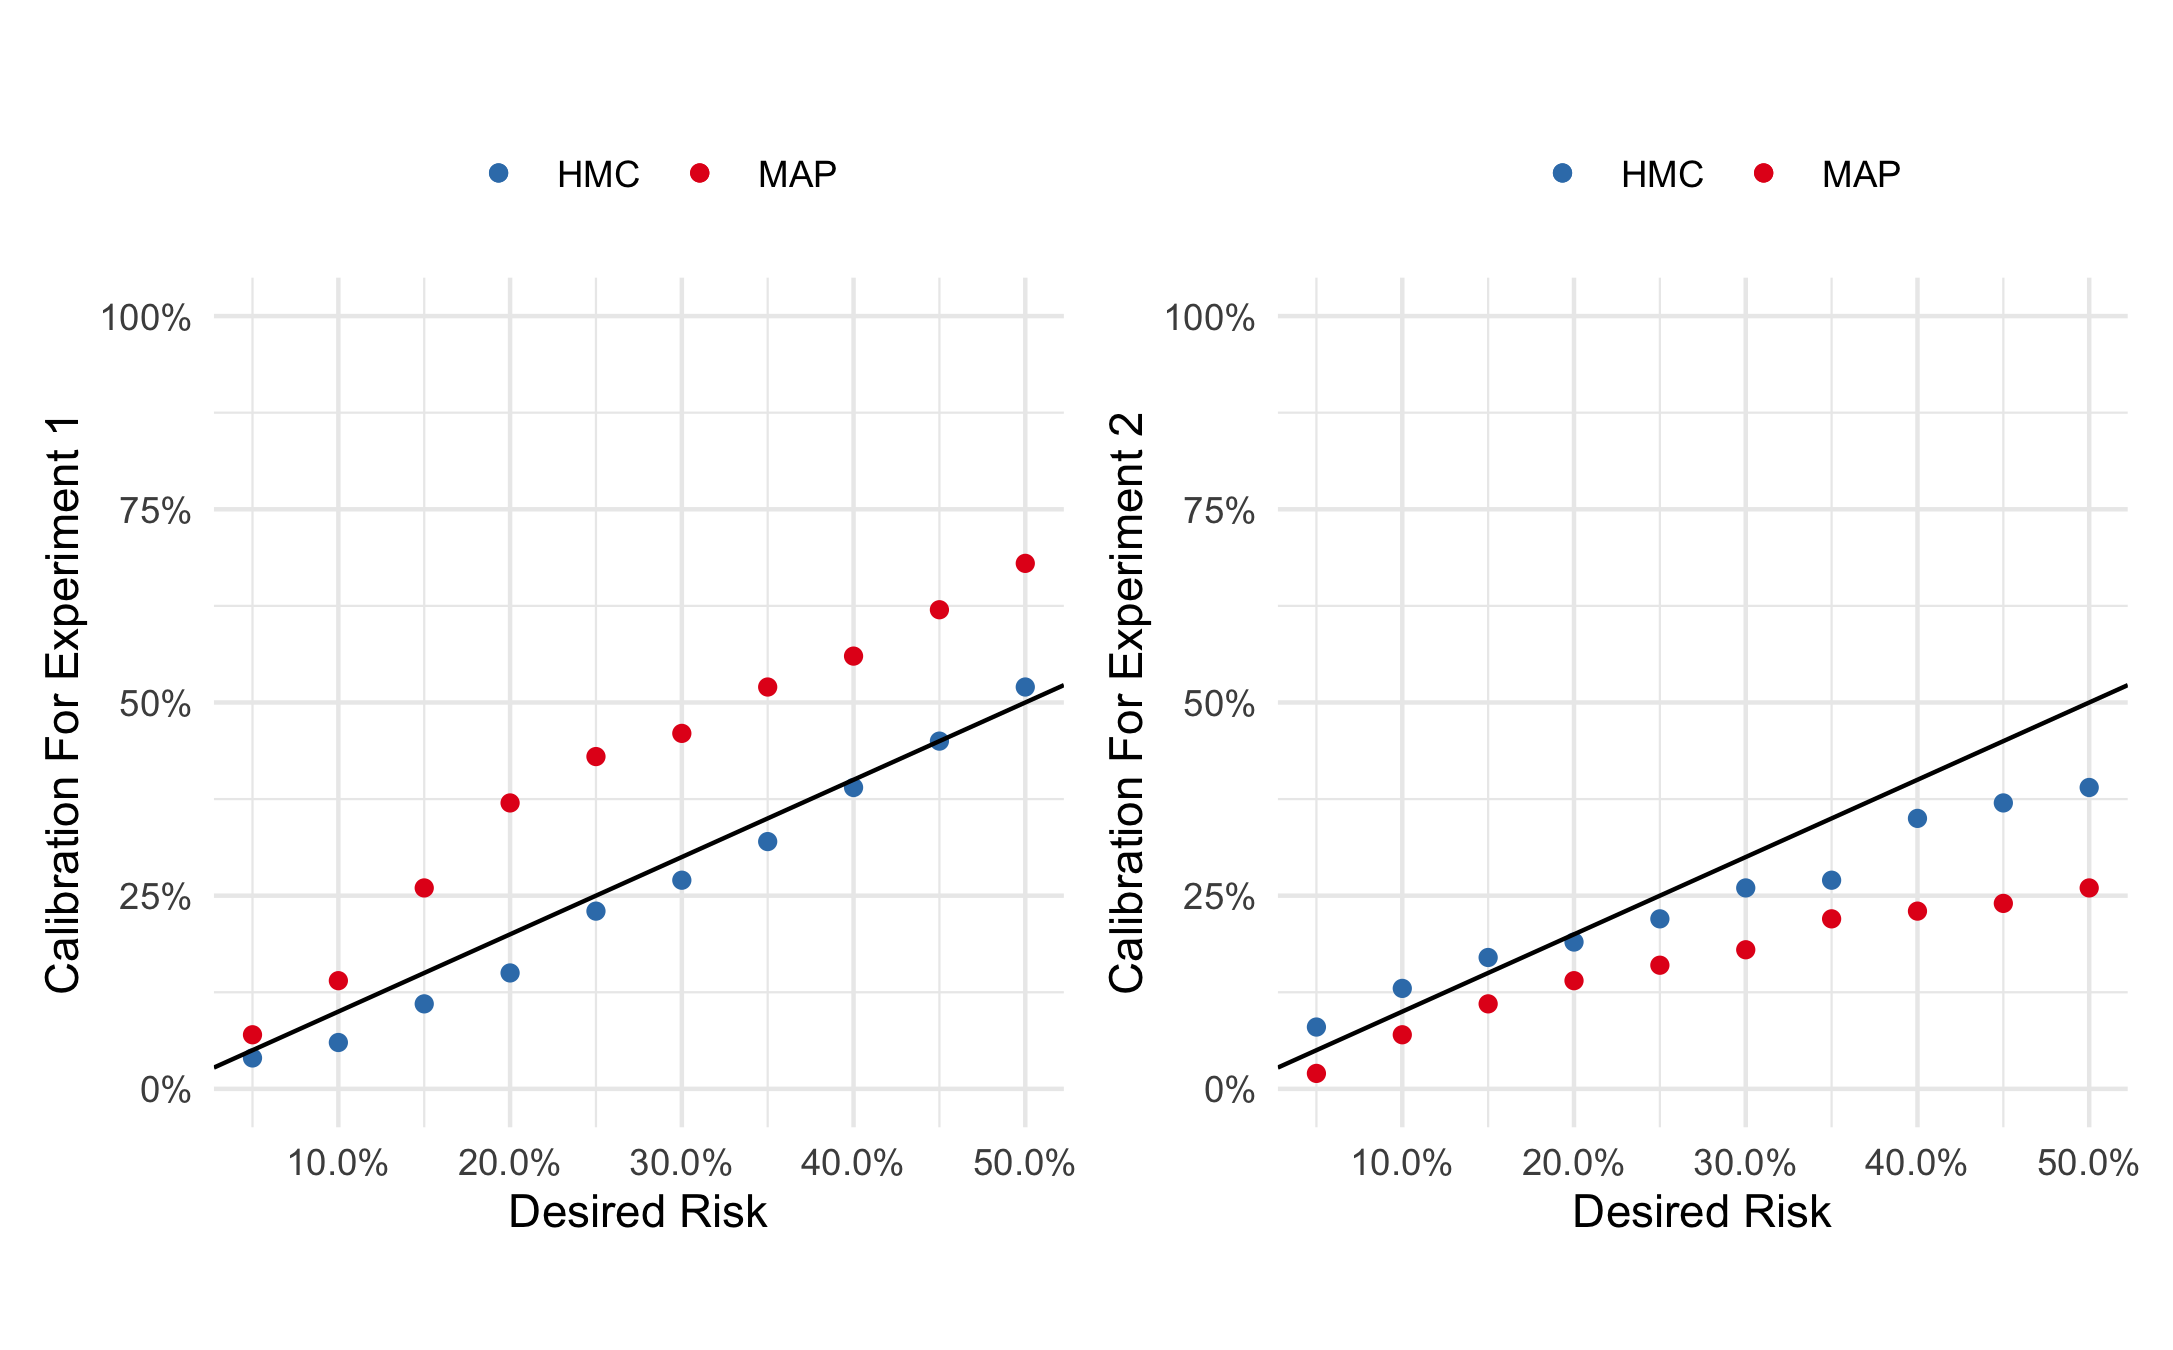
\includegraphics[width=\linewidth]{figs/fig8.png}
	\caption{Left: Calibration curves for assessing risk of being below 20 ng/ml.  Each dot represents the proportion of the 100 pseudopatients which fail to exceed the 20 ng/ml threshold.  When doses are chosen from samples obtained via HMC, then probabilities are well calibrated. When doses are chosen from samples obtained via MAP, more pseudopatients fail to exceed the threshold than were specified.  Right: Calibration curves for assessing risk of the max concentration being below 80 ng/ml. HMC appears to be better calibrated than MAP, though the calibration could stand to improve.}
	\label{fig:fig8}
\end{figure}



